\def\JClientAone{0.5}
\def\JManagerAone{0.75}
\def\JClientAtwo{0.5}
\def\JManagerAtwo{1}
\def\JClientBone{1}
\def\JManagerBone{0.5}
\def\JClientBtwo{1}
\def\JManagerBtwo{0.25}
\def\JClientCone{0.75}
\def\JManagerCone{0.5}
\def\JClientCtwo{0.75}
\def\JManagerCtwo{1}
\def\InitialDeterministic{42}
\def\RevisedDeterministic{42}
\def\CostDeterministic{0.0}
\def\CostLabelDeterministic{0.0000}
\def\InitialSingle{30}
\def\RevisedSingle{42}
\def\CostSingle{2.131419}
\def\CostLabelSingle{2.1314}
\def\InitialMulti{22}
\def\RevisedMulti{42}
\def\CostMulti{5.6347994}
\def\CostLabelMulti{5.6348}
\def\CostRatio{2.64}

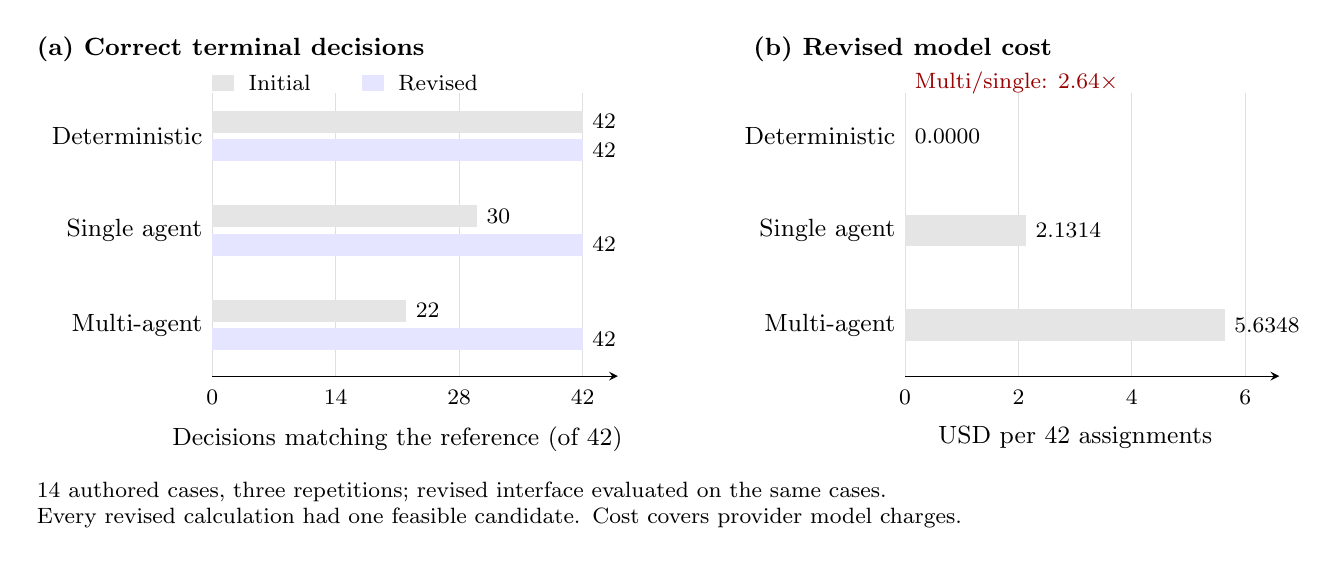
\begin{tikzpicture}[font=\small,>=stealth]
  \node[anchor=west,font=\small\bfseries] at (-2.35,4.65) {(a) Correct terminal decisions};
  \node[anchor=west,font=\small\bfseries] at (6.75,4.65) {(b) Revised model cost};
  \begin{scope}[x=0.112cm]
    \foreach \v in {0,14,28,42} {
      \draw[gray!25] (\v,0.5) -- (\v,4.1);
      \node[below,font=\footnotesize] at (\v,0.45) {\v};
    }
    \draw[->] (0,0.5) -- (46,0.5);
    \foreach \y/\name/\initial/\revised in {
      3.55/Deterministic/\InitialDeterministic/\RevisedDeterministic,
      2.35/Single agent/\InitialSingle/\RevisedSingle,
      1.15/Multi-agent/\InitialMulti/\RevisedMulti} {
      \node[left] at (0,\y) {\name};
      \fill[fill=gray!20] (0,\y+0.04) rectangle (\initial,\y+0.32);
      \fill[fill=blue!10] (0,\y-0.32) rectangle (\revised,\y-0.04);
      \node[right,font=\footnotesize] at (\initial,\y+0.18) {\initial};
      \node[right,font=\footnotesize] at (\revised,\y-0.18) {\revised};
    }
    \node[below] at (21,-0.02) {Decisions matching the reference (of 42)};
  \end{scope}
  \fill[fill=gray!20] (0,4.12) rectangle (0.28,4.32);
  \node[anchor=west,font=\footnotesize] at (0.34,4.22) {Initial};
  \fill[fill=blue!10] (1.9,4.12) rectangle (2.18,4.32);
  \node[anchor=west,font=\footnotesize] at (2.24,4.22) {Revised};
  \begin{scope}[shift={(8.8,0)},x=0.72cm]
    \foreach \v in {0,2,4,6} {
      \draw[gray!25] (\v,0.5) -- (\v,4.1);
      \node[below,font=\footnotesize] at (\v,0.45) {\v};
    }
    \draw[->] (0,0.5) -- (6.6,0.5);
    \foreach \y/\name/\cost/\label in {
      3.55/Deterministic/\CostDeterministic/\CostLabelDeterministic,
      2.35/Single agent/\CostSingle/\CostLabelSingle,
      1.15/Multi-agent/\CostMulti/\CostLabelMulti} {
      \node[left] at (0,\y) {\name};
      \fill[fill=gray!20] (0,\y-0.2) rectangle (\cost,\y+0.2);
      \node[right,font=\footnotesize] at (\cost,\y) {\label};
    }
    \node[below] at (3,-0.02) {USD per 42 assignments};
    \node[anchor=west,font=\footnotesize,text=red!60!black] at (0,4.22)
      {Multi/single: $\CostRatio\times$};
  \end{scope}
  \node[anchor=north west,align=left,font=\footnotesize,text width=15.9cm] at (-2.35,-0.72)
    {14 authored cases, three repetitions; revised interface evaluated on the same cases.\\
     Every revised calculation had one feasible candidate. Cost covers provider model charges.};
\end{tikzpicture}
